\chapter{Fluoroscopy}
\label{ch:fluoroscopy}

% Chapter-opening illustrated modality infographic.
\begin{center}
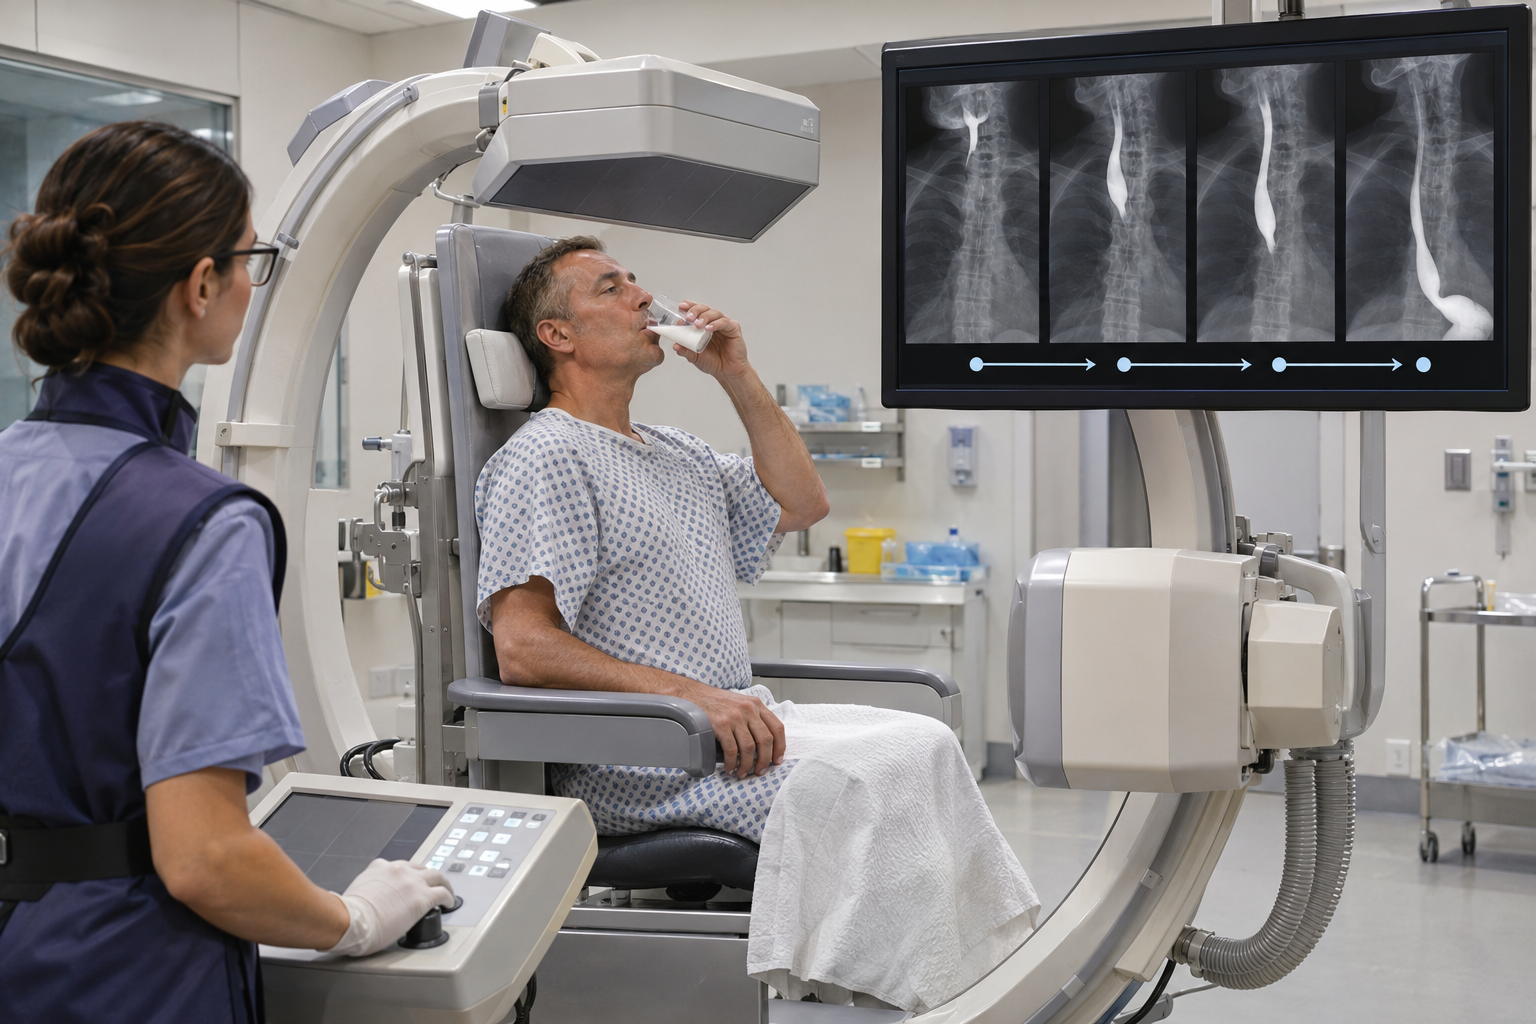
\includegraphics[width=\textwidth,keepaspectratio]{modalities/infographics/fluoroscopy_realistic.png}
\end{center}
\begin{center}\footnotesize Fluoroscopy captures X-ray images over time to show motion, contrast transit, or device movement; the sequence carries radiation exposure. AI-generated illustration; monitor images are not clinical studies.\end{center}

\section{Overview}
Fluoroscopy records a sequence of X-ray images. During a swallow, for example, the images show whether contrast passes below the vocal folds and whether this happens before, during, or after the swallow. A single frame may show the contrast in the airway but miss how it got there.

\section{Where fluoroscopy is used}
The 100 entries below describe diseases, structural abnormalities, and events observed during an examination. Some overlap. The entries include selected and historical uses alongside examinations in current routine practice. In angiography and arthrography, the findings described are visible on the contrast X-ray images themselves. An injection performed under fluoroscopy for a subsequent CT or MRI study serves a different purpose.

\subsection{Esophagus}
\textbf{Examinations.} A barium esophagram assesses contour and transit. A dedicated leak esophagram for suspected perforation often begins with water-soluble contrast. A negative initial study can miss a small leak.

\begin{enumerate}[leftmargin=*,itemsep=0.45em,topsep=0.4em]
\item \textbf{Achalasia.}\par\noindent\textbf{Why order fluoroscopy:} Dysphagia to liquids and solids, regurgitation, or unexplained esophageal retention may prompt a timed barium esophagram.\par\noindent\textbf{What to look for:} Smooth distal tapering, delayed emptying, and retained barium.\par\noindent\textbf{Role and sufficiency:} The study can strongly suggest achalasia and quantify emptying, but manometry confirms the motor disorder and endoscopy excludes a mechanical obstruction.
\item \textbf{Distal esophageal spasm.}\par\noindent\textbf{Why order fluoroscopy:} Intermittent dysphagia or noncardiac chest pain may lead to a dynamic esophagram.\par\noindent\textbf{What to look for:} Premature, nonpropulsive contractions and an intermittent corkscrew contour.\par\noindent\textbf{Role and sufficiency:} A normal study between episodes does not exclude spasm; high-resolution manometry is needed to establish the motility diagnosis.
\item \textbf{Epiphrenic diverticulum.}\par\noindent\textbf{Why order fluoroscopy:} Dysphagia, regurgitation, or retained food may prompt a barium study.\par\noindent\textbf{What to look for:} A contrast-filled pouch arising from the distal esophagus and its emptying.\par\noindent\textbf{Role and sufficiency:} Fluoroscopy usually demonstrates the pouch, but associated motility disorders require manometric assessment.
\item \textbf{Esophageal carcinoma.}\par\noindent\textbf{Why order fluoroscopy:} Progressive dysphagia, painful swallowing, or weight loss may prompt an esophagram when luminal narrowing is suspected.\par\noindent\textbf{What to look for:} Irregular shouldered narrowing, mucosal destruction, or a filling defect.\par\noindent\textbf{Role and sufficiency:} The study localizes and characterizes obstruction but cannot establish cancer; endoscopy with biopsy is required.
\item \textbf{Esophageal dysmotility.}\par\noindent\textbf{Why order fluoroscopy:} Swallowing difficulty, regurgitation, or unexplained transit symptoms may prompt real-time assessment.\par\noindent\textbf{What to look for:} Weak or disordered contractions, delayed clearance, and retained contrast.\par\noindent\textbf{Role and sufficiency:} It shows bolus transit during the sampled examination, but intermittent symptoms may not occur and manometry defines many specific motor disorders.
\item \textbf{Esophageal fistula.}\par\noindent\textbf{Why order fluoroscopy:} Coughing with swallowing, recurrent aspiration, or suspected communication after surgery or infection may prompt a contrast study.\par\noindent\textbf{What to look for:} Contrast passing through an abnormal tract into the airway or another organ.\par\noindent\textbf{Role and sufficiency:} Demonstrating the tract can establish its presence and location; a small or intermittently sealed fistula may be missed, requiring CT or endoscopy.
\item \textbf{Esophageal perforation.}\par\noindent\textbf{Why order fluoroscopy:} Severe chest pain after vomiting, instrumentation, or trauma raises urgent concern for a leak.\par\noindent\textbf{What to look for:} Extraluminal contrast, the leak site, and any contained collection.\par\noindent\textbf{Role and sufficiency:} A positive study demonstrates leakage, but a negative examination does not fully exclude a small perforation; CT and clinical assessment are used when suspicion remains.
\item \textbf{Esophageal stricture.}\par\noindent\textbf{Why order fluoroscopy:} Solid-food dysphagia or food impaction may prompt measurement of a narrowed segment.\par\noindent\textbf{What to look for:} Persistent narrowing, its length, contour, and effect on bolus passage.\par\noindent\textbf{Role and sufficiency:} Fluoroscopy maps the lumen but usually cannot determine the cause; endoscopy and biopsy may be needed, particularly for new or irregular strictures.
\item \textbf{Esophageal web.}\par\noindent\textbf{Why order fluoroscopy:} Intermittent solid-food dysphagia may prompt a targeted cervical esophagram.\par\noindent\textbf{What to look for:} A thin shelf-like filling defect, often anterior and proximal.\par\noindent\textbf{Role and sufficiency:} A well-positioned study can show the web; subtle lesions may be missed without appropriate views and distension.
\item \textbf{Gastroesophageal reflux.}\par\noindent\textbf{Why order fluoroscopy:} Reflux symptoms may lead to evaluation for anatomy or associated complications, not to prove ordinary reflux episodes.\par\noindent\textbf{What to look for:} Reflux observed during the examination, hiatal hernia, or stricture.\par\noindent\textbf{Role and sufficiency:} Reflux may occur in healthy people and may be absent during the brief study; fluoroscopy alone neither confirms nor excludes GERD.
\item \textbf{Hiatal hernia.}\par\noindent\textbf{Why order fluoroscopy:} Dysphagia, reflux symptoms, or suspected intrathoracic stomach may prompt a dynamic upper GI study.\par\noindent\textbf{What to look for:} Stomach above the diaphragm and the position of the gastroesophageal junction.\par\noindent\textbf{Role and sufficiency:} Fluoroscopy can demonstrate and classify many hernias, though size can vary with position and strain; CT or endoscopy may be used for complications.
\item \textbf{Schatzki ring.}\par\noindent\textbf{Why order fluoroscopy:} Intermittent solid-food sticking or food impaction may prompt a distended esophagram.\par\noindent\textbf{What to look for:} A thin circumferential ring at the gastroesophageal junction and narrowing of the lumen.\par\noindent\textbf{Role and sufficiency:} A properly performed study often shows the ring, but endoscopy may be needed when symptoms persist or treatment is planned.
\item \textbf{Zenker diverticulum.}\par\noindent\textbf{Why order fluoroscopy:} Oropharyngeal dysphagia, regurgitation of undigested food, halitosis, or cough after eating may prompt a pharyngoesophagram.\par\noindent\textbf{What to look for:} A posterior pouch above the cricopharyngeus, its size, and retention or aspiration of contrast.\par\noindent\textbf{Role and sufficiency:} Fluoroscopy usually defines the pouch and swallowing mechanics; endoscopy is not a substitute for initial anatomic mapping and should be approached cautiously.
\end{enumerate}

\subsection{Oropharyngeal swallowing disorders}
\textbf{Examinations.} Videofluoroscopic swallowing study (VFSS), modified barium swallow.

\begin{enumerate}[leftmargin=*,itemsep=0.45em,topsep=0.4em]
\item \textbf{Cricopharyngeal dysfunction.}\par\noindent\textbf{Why order VFSS:} A sensation of food sticking in the throat, repeated swallows, or post-swallow residue may prompt dynamic swallowing assessment.\par\noindent\textbf{What to look for:} Reduced opening of the pharyngoesophageal segment, bolus hold-up, and residue.\par\noindent\textbf{Role and sufficiency:} VFSS shows the movement pattern but not every cause of impaired opening; clinical swallowing assessment and sometimes endoscopy/manometry add context.
\item \textbf{Delayed initiation of the pharyngeal swallow.}\par\noindent\textbf{Why order VFSS:} Coughing, choking, or delayed swallowing with meals may prompt evaluation of swallow timing.\par\noindent\textbf{What to look for:} Bolus entering the pharynx before the swallow response begins, interpreted relative to bolus consistency and location.\par\noindent\textbf{Role and sufficiency:} VFSS directly observes sampled swallows, but results vary with task and bolus; it does not by itself identify the neurologic or muscular cause.
\item \textbf{Laryngeal penetration.}\par\noindent\textbf{Why order VFSS:} Coughing or a wet voice during meals may prompt assessment of airway protection.\par\noindent\textbf{What to look for:} Contrast entering the laryngeal vestibule but remaining above the vocal folds; record depth and whether it clears.\par\noindent\textbf{Role and sufficiency:} VFSS identifies penetration during tested swallows, but a limited sample cannot guarantee safety with every food or meal.
\item \textbf{Oropharyngeal dysphagia.}\par\noindent\textbf{Why order VFSS:} Difficulty initiating a swallow, coughing with liquids, nasal regurgitation, or unexplained aspiration may prompt videofluoroscopy.\par\noindent\textbf{What to look for:} Oral transfer, swallow timing, pharyngeal clearance, airway entry, and upper esophageal opening.\par\noindent\textbf{Role and sufficiency:} VFSS characterizes mechanics and helps guide diet or therapy; it does not alone establish the underlying disease or represent every meal.
\item \textbf{Pharyngeal muscle weakness.}\par\noindent\textbf{Why order VFSS:} Weak cough, repeated swallows, or a sensation of residue may prompt functional assessment.\par\noindent\textbf{What to look for:} Reduced pharyngeal constriction and retained contrast after the swallow.\par\noindent\textbf{Role and sufficiency:} Residue supports impaired clearance but is nonspecific; correlate with examination, neurologic history, and other swallowing findings.
\item \textbf{Pulmonary aspiration.}\par\noindent\textbf{Why order VFSS:} Coughing, choking, recurrent chest infections, or suspected silent aspiration may prompt a videofluoroscopic swallow study.\par\noindent\textbf{What to look for:} Contrast passing below the vocal folds, including timing and whether it is expelled.\par\noindent\textbf{Role and sufficiency:} Aspiration observed during the test confirms airway entry for that sampled swallow, but a negative study cannot exclude intermittent aspiration in other conditions or at other times.
\item \textbf{Velopharyngeal insufficiency.}\par\noindent\textbf{Why order VFSS:} Nasal escape of liquids, hypernasal speech, or swallowing difficulty may prompt dynamic assessment.\par\noindent\textbf{What to look for:} Contrast entering the nasopharynx through incomplete velopharyngeal closure.\par\noindent\textbf{Role and sufficiency:} Fluoroscopy demonstrates closure during the tested task; speech-language assessment and targeted ENT evaluation determine functional impact and cause.
\end{enumerate}

\subsection{Stomach and duodenum}
\textbf{Examination.} Upper gastrointestinal contrast series.

\begin{enumerate}[leftmargin=*,itemsep=0.45em,topsep=0.4em]
\item \textbf{Annular pancreas.}\par\noindent\textbf{Why order fluoroscopy:} Recurrent vomiting or duodenal obstruction, especially in an infant, may prompt an upper GI series.\par\noindent\textbf{What to look for:} Fixed narrowing of the second duodenal portion and delayed passage.\par\noindent\textbf{Role and sufficiency:} The narrowing is an indirect sign; CT or MRI can demonstrate pancreatic tissue encircling the duodenum and define anatomy.
\item \textbf{Duodenal diverticulum.}\par\noindent\textbf{Why order fluoroscopy:} Postprandial discomfort, bleeding, or suspected obstruction may prompt luminal assessment.\par\noindent\textbf{What to look for:} A contrast-filled pouch communicating with the duodenal lumen, including its neck and position.\par\noindent\textbf{Role and sufficiency:} Fluoroscopy can establish a patent diverticulum, but cross-sectional imaging or endoscopy may be needed for complications or an uncertain cause of symptoms.
\item \textbf{Duodenal stenosis.}\par\noindent\textbf{Why order fluoroscopy:} Persistent vomiting or suspected proximal small-bowel obstruction may prompt an upper GI series.\par\noindent\textbf{What to look for:} The level, length, and severity of fixed narrowing and upstream hold-up.\par\noindent\textbf{Role and sufficiency:} It maps luminal transit but may not identify the cause; endoscopy or CT/MRI is used when a mass or extrinsic compression is suspected.
\item \textbf{Duodenal ulcer.}\par\noindent\textbf{Why order fluoroscopy:} Epigastric pain or suspected ulcer-related deformity may lead to contrast examination when endoscopy is unavailable or unsuitable.\par\noindent\textbf{What to look for:} A niche projecting beyond the expected contour, with bulb deformity or scarring.\par\noindent\textbf{Role and sufficiency:} Fluoroscopy may show an ulcer but cannot biopsy or reliably exclude malignancy; endoscopy is preferred for diagnosis and sampling.
\item \textbf{Gastric carcinoma.}\par\noindent\textbf{Why order fluoroscopy:} Early satiety, weight loss, anemia, or persistent vomiting may prompt evaluation of gastric contour if an upper GI series is selected.\par\noindent\textbf{What to look for:} Irregular filling defect, shouldered narrowing, rigidity, or poor distensibility.\par\noindent\textbf{Role and sufficiency:} These findings raise suspicion but are not diagnostic; endoscopy with biopsy is required.
\item \textbf{Gastric diverticulum.}\par\noindent\textbf{Why order fluoroscopy:} A suspected anatomic pouch in a patient with upper abdominal symptoms may prompt an upper GI series.\par\noindent\textbf{What to look for:} A contrast-filled outpouching, usually near the gastric fundus, in more than one projection.\par\noindent\textbf{Role and sufficiency:} Fluoroscopy can demonstrate a communicating pouch; CT may clarify its location or distinguish it from an adjacent lesion.
\item \textbf{Gastric outlet obstruction.}\par\noindent\textbf{Why order fluoroscopy:} Recurrent nonbilious vomiting, early satiety, or gastric distension may prompt assessment of passage through the pylorus.\par\noindent\textbf{What to look for:} Persistent hold-up, narrowing, and the level of transition rather than delayed emptying alone.\par\noindent\textbf{Role and sufficiency:} It confirms impaired transit during the study but may not determine the cause; endoscopy and cross-sectional imaging assess structural disease.
\item \textbf{Gastric ulcer.}\par\noindent\textbf{Why order fluoroscopy:} Persistent epigastric pain or suspected ulcer-related deformity may prompt an upper GI contrast study in selected settings.\par\noindent\textbf{What to look for:} Contrast pooling in a crater, surrounding folds, and any mass-like or irregular contour.\par\noindent\textbf{Role and sufficiency:} It cannot provide tissue diagnosis or reliably distinguish benign from malignant ulceration; endoscopy with biopsy is needed when indicated.
\item \textbf{Gastric volvulus.}\par\noindent\textbf{Why order fluoroscopy:} Acute epigastric or chest pain with retching and inability to pass a tube can raise concern for volvulus.\par\noindent\textbf{What to look for:} Abnormal gastric axis, compartmentalization, beaking, and obstruction at the outlet.\par\noindent\textbf{Role and sufficiency:} An upper GI series can demonstrate rotation and impaired passage in a stable patient; urgent CT and clinical assessment define complications such as ischemia or perforation.
\item \textbf{Intestinal malrotation.}\par\noindent\textbf{Why order fluoroscopy:} Bilious vomiting in an infant or intermittent obstructive symptoms may prompt urgent upper GI evaluation.\par\noindent\textbf{What to look for:} Course of the duodenum and position of the duodenojejunal junction, with attention to corkscrew configuration.\par\noindent\textbf{Role and sufficiency:} A technically adequate study is the principal luminal test, but equivocal results require expert review and often ultrasound or cross-sectional imaging; do not delay urgent surgical assessment when volvulus is suspected.
\item \textbf{Linitis plastica.}\par\noindent\textbf{Why order fluoroscopy:} Early satiety, weight loss, or suspected infiltrative gastric disease may prompt assessment of distensibility.\par\noindent\textbf{What to look for:} Diffuse narrowing, rigid poorly distensible stomach, and thickened folds.\par\noindent\textbf{Role and sufficiency:} The pattern suggests infiltration but cannot establish its cause; endoscopic biopsies, sometimes repeated or obtained with EUS, are needed.
\item \textbf{Midgut volvulus.}\par\noindent\textbf{Why order fluoroscopy:} Acute bilious vomiting and suspected malrotation-related obstruction demand urgent evaluation.\par\noindent\textbf{What to look for:} Abnormally positioned duodenojejunal junction and corkscrew twisting of the duodenum or proximal jejunum.\par\noindent\textbf{Role and sufficiency:} Fluoroscopy can identify the characteristic configuration, but urgent management is driven by the clinical picture and surgical assessment; a negative or equivocal study does not safely exclude volvulus if suspicion remains high.
\item \textbf{Superior mesenteric artery syndrome.}\par\noindent\textbf{Why order fluoroscopy:} Postprandial pain, early satiety, and bilious vomiting, particularly after weight loss, may prompt assessment of duodenal transit.\par\noindent\textbf{What to look for:} Compression at the third duodenal portion, proximal dilatation, and improved passage with position change.\par\noindent\textbf{Role and sufficiency:} Fluoroscopy demonstrates functional obstruction but does not prove vascular compression; CT or MRI measures the aortomesenteric relationship and excludes other causes.
\end{enumerate}

\subsection{Small intestine}
\textbf{Examinations.} Small bowel follow-through and enteroclysis examine the lumen. In selected patients with known obstruction, a water-soluble contrast challenge assesses progression to the colon. CT generally evaluates the site, cause, and complications of acute obstruction.

\begin{enumerate}[leftmargin=*,itemsep=0.45em,topsep=0.4em]
\item \textbf{Crohn disease.}\par\noindent\textbf{Why order fluoroscopy:} Chronic diarrhea, abdominal pain, or suspected stricture may prompt small-bowel contrast evaluation when enterography is unavailable or for selected transit questions.\par\noindent\textbf{What to look for:} Skip areas, aphthous or longitudinal ulcers, cobblestoning, and fixed narrowing such as a string sign.\par\noindent\textbf{Role and sufficiency:} It depicts mucosal contour and strictures but not transmural complications well; CT or MR enterography and endoscopy are generally more comprehensive.
\item \textbf{Small bowel diverticulosis.}\par\noindent\textbf{Why order fluoroscopy:} Unexplained anemia, pain, or suspected diverticular anatomy may prompt a small-bowel series.\par\noindent\textbf{What to look for:} One or more contrast-filled outpouchings arising from the bowel, distinguished from overlapping loops by tracking them across views.\par\noindent\textbf{Role and sufficiency:} Fluoroscopy can show communicating diverticula but may miss complications or lesions outside the lumen; CT is used for suspected inflammation or bleeding complications.
\item \textbf{Small bowel dysmotility.}\par\noindent\textbf{Why order fluoroscopy:} Persistent bloating, vomiting, or transit symptoms after mechanical obstruction is considered may prompt a timed small-bowel study.\par\noindent\textbf{What to look for:} Delayed progression, ineffective propulsion, or disorganized transit across serial images.\par\noindent\textbf{Role and sufficiency:} Transit is affected by preparation, medications, and technique; fluoroscopy suggests abnormal motility but does not specify its cause or replace targeted physiological testing.
\item \textbf{Small bowel fistula.}\par\noindent\textbf{Why order fluoroscopy:} Drainage, recurrent infection, or suspected communication after surgery or inflammatory disease may prompt contrast evaluation.\par\noindent\textbf{What to look for:} Contrast traversing an abnormal tract between loops or into an adjacent organ.\par\noindent\textbf{Role and sufficiency:} A visible tract confirms communication during the study, but intermittent or narrow fistulas may not opacify; CT/MR enterography or endoscopy can provide additional mapping.
\item \textbf{Small bowel obstruction.}\par\noindent\textbf{Why order fluoroscopy:} Vomiting, distension, and failure to pass stool or gas may prompt a water-soluble contrast challenge in selected patients with suspected adhesive obstruction.\par\noindent\textbf{What to look for:} Delayed passage at a transition and whether contrast reaches the colon within the protocol interval.\par\noindent\textbf{Role and sufficiency:} The challenge helps assess progression but does not reliably identify the cause or complications; CT is generally used to locate the transition and evaluate ischemia or closed loop.
\item \textbf{Small bowel strictures.}\par\noindent\textbf{Why order fluoroscopy:} Intermittent obstructive symptoms or known inflammatory disease may prompt mapping of a narrowed segment.\par\noindent\textbf{What to look for:} Persistent focal or multifocal narrowing, length, upstream dilatation, and transit delay.\par\noindent\textbf{Role and sufficiency:} It demonstrates luminal caliber but cannot reliably distinguish inflammatory from fibrotic narrowing or show extraluminal disease; enterography and endoscopy may be needed.
\item \textbf{Small bowel tumors.}\par\noindent\textbf{Why order fluoroscopy:} Occult bleeding, anemia, or unexplained obstructive symptoms may prompt evaluation of the small-bowel lumen.\par\noindent\textbf{What to look for:} Persistent filling defect, irregular narrowing, mucosal destruction, or shouldering.\par\noindent\textbf{Role and sufficiency:} A mass can be localized, but fluoroscopy cannot determine histology or fully stage it; capsule/deep enteroscopy and CT or MR enterography are selected according to the clinical question.
\end{enumerate}

\subsection{Colon and rectum}
\textbf{Examination.} Contrast enema. Water-soluble contrast is used when evaluating a suspected postoperative leak. In children with suspected ileocolic intussusception, ultrasound is usually the first examination. A fluoroscopic air or liquid enema can show the intussusception and document its reduction.

\begin{enumerate}[leftmargin=*,itemsep=0.45em,topsep=0.4em]
\item \textbf{Colonic anastomotic leakage.}\par\noindent\textbf{Why order fluoroscopy:} Fever, pain, or concerning drain output after colorectal surgery may prompt a water-soluble contrast enema to assess an anastomosis.\par\noindent\textbf{What to look for:} Contrast outside the bowel at the surgical join and the extent of any contained leak.\par\noindent\textbf{Role and sufficiency:} A demonstrated leak is useful, but small or intermittently sealed defects may be missed; CT with appropriate contrast and clinical assessment are needed when suspicion persists.
\item \textbf{Colonic diverticulosis.}\par\noindent\textbf{Why order fluoroscopy:} A contrast enema may demonstrate diverticula when luminal anatomy is being assessed for another reason.\par\noindent\textbf{What to look for:} Multiple small contrast-filled outpouchings beyond the expected colonic contour.\par\noindent\textbf{Role and sufficiency:} It can establish diverticular anatomy but does not diagnose acute diverticulitis or explain bleeding; CT or endoscopy is selected for those questions.
\item \textbf{Colonic fistula.}\par\noindent\textbf{Why order fluoroscopy:} Fecaluria, pneumaturia, vaginal stool passage, or persistent drainage may prompt a targeted contrast study.\par\noindent\textbf{What to look for:} Contrast crossing from colon into an adjacent organ or tract.\par\noindent\textbf{Role and sufficiency:} Direct opacification confirms communication, but a narrow or intermittently patent fistula may be missed; CT and endoscopy help identify the cause and surrounding disease.
\item \textbf{Colonic strictures.}\par\noindent\textbf{Why order fluoroscopy:} Altered bowel habits, obstructive symptoms, or postoperative narrowing may prompt luminal mapping.\par\noindent\textbf{What to look for:} Fixed narrowing, length, contour, and proximal dilatation.\par\noindent\textbf{Role and sufficiency:} The enema defines caliber but not etiology; colonoscopy with biopsy or CT is required when malignancy or extrinsic disease is possible.
\item \textbf{Colorectal carcinoma.}\par\noindent\textbf{Why order fluoroscopy:} Obstructive symptoms may lead to contrast evaluation when colonoscopy cannot traverse a narrowing or is not feasible.\par\noindent\textbf{What to look for:} Short irregular shouldered narrowing, annular constriction, or persistent filling defect.\par\noindent\textbf{Role and sufficiency:} These signs suggest a tumor but cannot establish histology; colonoscopy and biopsy are needed, and CT stages disease.
\item \textbf{Hirschsprung disease.}\par\noindent\textbf{Why order fluoroscopy:} Delayed passage of meconium, abdominal distension, and bilious vomiting in an infant may prompt a contrast enema after stabilization.\par\noindent\textbf{What to look for:} A narrow distal aganglionic segment with a transition to dilated proximal colon and a reversed rectosigmoid ratio.\par\noindent\textbf{Role and sufficiency:} The enema supports localization, but a normal study does not exclude disease; rectal suction biopsy establishes the diagnosis.
\item \textbf{Meconium ileus.}\par\noindent\textbf{Why order fluoroscopy:} A newborn with distal bowel obstruction and failure to pass meconium may undergo a water-soluble contrast enema, which can also be therapeutic.\par\noindent\textbf{What to look for:} Microcolon and terminal ileal filling defects from inspissated meconium.\par\noindent\textbf{Role and sufficiency:} The pattern supports meconium ileus but microcolon is not specific; clinical assessment and evaluation for cystic fibrosis are important.
\item \textbf{Neonatal small left colon syndrome.}\par\noindent\textbf{Why order fluoroscopy:} A newborn with abdominal distension and delayed stool passage may undergo contrast enema to assess distal obstruction.\par\noindent\textbf{What to look for:} A narrow descending colon and sigmoid with an abrupt caliber change near the splenic flexure.\par\noindent\textbf{Role and sufficiency:} The appearance supports the diagnosis and the enema may relieve obstruction, but clinical course and exclusion of Hirschsprung disease are needed if symptoms persist.
\item \textbf{Pediatric ileocolic intussusception.}\par\noindent\textbf{Why order fluoroscopy:} Episodic severe abdominal pain, vomiting, lethargy, or bloody stool after ultrasound suggests intussusception may prompt image-guided enema reduction.\par\noindent\textbf{What to look for:} A meniscus or coiled-spring filling defect and, during treatment, reflux of contrast into the terminal ileum indicating reduction.\par\noindent\textbf{Role and sufficiency:} Enema is diagnostic and therapeutic in suitable stable patients; perforation or peritonitis changes management, and ultrasound is generally the initial diagnostic examination.
\item \textbf{Sigmoid volvulus.}\par\noindent\textbf{Why order fluoroscopy:} Marked distension, constipation, and obstructive symptoms may prompt contrast enema in a stable patient when decompression is being considered.\par\noindent\textbf{What to look for:} Smooth tapering to a bird-beak at the twist and failure of contrast to pass.\par\noindent\textbf{Role and sufficiency:} It can show the level and sometimes aid decompression, but CT is commonly used to assess ischemia or perforation; peritonitis or suspected bowel compromise requires urgent surgical evaluation.
\item \textbf{Ulcerative colitis.}\par\noindent\textbf{Why order fluoroscopy:} Contrast enema now has limited use and may be considered only for selected structural questions outside acute severe colitis.\par\noindent\textbf{What to look for:} Chronic loss of haustra, shortening, and a featureless lead-pipe contour.\par\noindent\textbf{Role and sufficiency:} These are chronic changes, not a reliable measure of active inflammation; endoscopy with biopsy and clinical assessment guide diagnosis, while barium enema is generally avoided in severe acute disease.
\end{enumerate}

\subsection{Pelvic floor and defecation disorders}
\textbf{Examination.} Fluoroscopic defecography.

\begin{enumerate}[leftmargin=*,itemsep=0.45em,topsep=0.4em]
\item \textbf{Descending perineum syndrome.}\par\noindent\textbf{Why order fluoroscopy:} Excessive straining, incomplete evacuation, or pelvic pressure may prompt defecography.\par\noindent\textbf{What to look for:} Abnormally large perineal descent during strain and evacuation, measured relative to a fixed pelvic line.\par\noindent\textbf{Role and sufficiency:} Defecography documents movement during the test but descent can occur in asymptomatic people; symptoms and anorectal examination determine relevance.
\item \textbf{Dyssynergic defecation.}\par\noindent\textbf{Why order fluoroscopy:} Chronic straining, prolonged toileting, and incomplete evacuation may prompt assessment of coordinated evacuation.\par\noindent\textbf{What to look for:} Failure of the anorectal angle to open, paradoxical narrowing, and retained rectal contrast.\par\noindent\textbf{Role and sufficiency:} Defecography can demonstrate an abnormal pattern, but diagnosis requires compatible symptoms and is usually corroborated with anorectal manometry and balloon expulsion testing.
\item \textbf{Enterocele.}\par\noindent\textbf{Why order fluoroscopy:} Pelvic pressure or obstructed defecation, especially after pelvic surgery, may prompt evacuation imaging.\par\noindent\textbf{What to look for:} Small bowel descending between rectum and vagina during strain; oral contrast can distinguish bowel loops.\par\noindent\textbf{Role and sufficiency:} Defecography shows dynamic descent and its relation to evacuation, but clinical significance depends on symptoms and may require pelvic MRI for broader compartment assessment.
\item \textbf{Rectal intussusception.}\par\noindent\textbf{Why order fluoroscopy:} Obstructed defecation, tenesmus, or incomplete emptying may prompt dynamic evaluation.\par\noindent\textbf{What to look for:} Rectal wall telescoping inward during evacuation and whether it obstructs the outlet.\par\noindent\textbf{Role and sufficiency:} Defecography depicts the event under test conditions, but minor intussusception may be incidental; correlate with symptoms and examination.
\item \textbf{Rectal prolapse.}\par\noindent\textbf{Why order fluoroscopy:} A history of tissue protrusion or obstructed evacuation may prompt defecography when examination does not capture the event.\par\noindent\textbf{What to look for:} Full-thickness rectal wall descending through the anal canal during evacuation.\par\noindent\textbf{Role and sufficiency:} Fluoroscopy can document dynamic prolapse, but visible external prolapse is often diagnosed clinically; the study helps define associated pelvic floor abnormalities.
\item \textbf{Rectocele.}\par\noindent\textbf{Why order fluoroscopy:} Vaginal splinting, incomplete evacuation, or a bulge sensation may prompt defecography.\par\noindent\textbf{What to look for:} Anterior rectal wall pouching into the vagina, its depth, retained contrast, and emptying.\par\noindent\textbf{Role and sufficiency:} A small rectocele is common and may be incidental; imaging alone does not establish the cause of symptoms or need for treatment.
\item \textbf{Sigmoidocele.}\par\noindent\textbf{Why order fluoroscopy:} Pelvic pressure or difficult evacuation may prompt evaluation for a descending sigmoid loop.\par\noindent\textbf{What to look for:} Sigmoid colon entering the cul-de-sac during evacuation and compressing the rectum.\par\noindent\textbf{Role and sufficiency:} Defecography captures dynamic descent, while pelvic MRI can assess multiple compartments; findings require symptom correlation.
\end{enumerate}

\subsection{Urinary system}
\textbf{Examinations.} Voiding cystourethrography (VCUG), retrograde urethrography, retrograde cystography, and video-urodynamics.

\begin{enumerate}[leftmargin=*,itemsep=0.45em,topsep=0.4em]
\item \textbf{Bladder diverticulum.}\par\noindent\textbf{Why order fluoroscopy:} Recurrent infection, incomplete emptying, or suspected outlet obstruction may prompt cystography or VCUG.\par\noindent\textbf{What to look for:} A contrast-filled pouch communicating with the bladder, its size, and residual contrast after voiding.\par\noindent\textbf{Role and sufficiency:} It demonstrates a patent diverticulum but does not determine why it formed; ultrasound, cystoscopy, or urodynamics may clarify associated dysfunction.
\item \textbf{Bladder outlet obstruction.}\par\noindent\textbf{Why order fluoroscopy:} Weak stream, straining, or retention may prompt video-urodynamic evaluation when the level or mechanism is uncertain.\par\noindent\textbf{What to look for:} Failure of the bladder neck or urethra to open normally and the level of narrowing during voiding.\par\noindent\textbf{Role and sufficiency:} Images localize anatomy, but pressure-flow measurements distinguish obstruction from weak detrusor contraction; fluoroscopy alone is insufficient.
\item \textbf{Bladder rupture.}\par\noindent\textbf{Why order fluoroscopy:} Pelvic trauma with hematuria or suspected postoperative injury may prompt retrograde cystography.\par\noindent\textbf{What to look for:} Contrast outside the bladder, within the peritoneal cavity or around the extraperitoneal pelvis, after adequate retrograde filling.\par\noindent\textbf{Role and sufficiency:} Properly performed cystography can demonstrate and classify rupture; passive excreted contrast may miss it, and CT cystography is commonly used in trauma.
\item \textbf{Detrusor-sphincter dyssynergia.}\par\noindent\textbf{Why order fluoroscopy:} Voiding difficulty in a patient with neurologic disease may prompt synchronized video-urodynamics.\par\noindent\textbf{What to look for:} Persistent or paradoxical outlet closure while the detrusor contracts, with interrupted flow or elevated pressure.\par\noindent\textbf{Role and sufficiency:} Fluoroscopy shows outlet behavior but diagnosis depends on synchronized pressure-flow testing and sometimes sphincter electromyography.
\item \textbf{Neurogenic bladder.}\par\noindent\textbf{Why order fluoroscopy:} Neurologic disease with incontinence, retention, recurrent infection, or upper-tract risk may prompt video-urodynamics.\par\noindent\textbf{What to look for:} Bladder contour, compliance-related changes, reflux, outlet coordination, and emptying during measured pressure and flow.\par\noindent\textbf{Role and sufficiency:} The radiographic contour is nonspecific; diagnosis and risk stratification require urodynamic measurements and clinical context.
\item \textbf{Posterior urethral valves.}\par\noindent\textbf{Why order fluoroscopy:} A male infant with poor urinary stream, antenatal hydronephrosis, or urinary infection may undergo VCUG.\par\noindent\textbf{What to look for:} Dilated posterior urethra with abrupt narrowing, bladder trabeculation, and possible reflux.\par\noindent\textbf{Role and sufficiency:} VCUG strongly suggests the obstruction, but cystoscopy confirms and treats the valves; a technically inadequate voiding phase can miss them.
\item \textbf{Urethral diverticulum.}\par\noindent\textbf{Why order fluoroscopy:} Recurrent infection, postvoid dribbling, or a periurethral mass may prompt voiding imaging.\par\noindent\textbf{What to look for:} A contrast-opacified side pouch communicating with the urethra.\par\noindent\textbf{Role and sufficiency:} A patent opening is required for visualization, so a negative study cannot exclude a closed or poorly filling diverticulum; MRI or endoscopy may be needed.
\item \textbf{Urethral rupture.}\par\noindent\textbf{Why order fluoroscopy:} Blood at the meatus, pelvic trauma, or suspected urethral injury may prompt retrograde urethrography before catheterization.\par\noindent\textbf{What to look for:} Contrast extravasation and whether it reaches the proximal urethra or bladder.\par\noindent\textbf{Role and sufficiency:} The study classifies the injury pattern, but does not replace trauma evaluation; avoid blind urethral catheterization when injury is suspected.
\item \textbf{Urethral stricture.}\par\noindent\textbf{Why order fluoroscopy:} Weak stream, retention, or recurrent infection may prompt retrograde urethrography for procedural planning.\par\noindent\textbf{What to look for:} Site, length, caliber, and number of narrowed segments, with proximal urethral filling where possible.\par\noindent\textbf{Role and sufficiency:} It maps luminal anatomy well but may not fully characterize spongiofibrosis; cystoscopy and clinical findings can complement it.
\item \textbf{Urinary fistula.}\par\noindent\textbf{Why order fluoroscopy:} Urine leaking through the vagina, skin, or bowel, or persistent postoperative drainage, may prompt targeted cystography or urethrography.\par\noindent\textbf{What to look for:} Contrast crossing an abnormal communication and the organs involved.\par\noindent\textbf{Role and sufficiency:} Opacification confirms a patent tract, but small or intermittent fistulas can be missed; CT, MRI, endoscopy, or examination may be required to map it.
\item \textbf{Vesicoureteral reflux.}\par\noindent\textbf{Why order fluoroscopy:} Recurrent febrile urinary infections or suspected reflux-related renal injury may prompt VCUG.\par\noindent\textbf{What to look for:} Retrograde contrast entering the ureter and renal collecting system during filling or voiding; grade the extent and persistence.\par\noindent\textbf{Role and sufficiency:} VCUG directly demonstrates reflux during the examination, but intermittent reflux can be missed and the study does not itself measure renal scarring or function.
\end{enumerate}

\subsection{Female reproductive system}
\textbf{Examination.} Hysterosalpingography (HSG) outlines the uterine cavity and communicating tubes. A divided cavity can occur with either a septate or a bicornuate uterus. Three-dimensional transvaginal ultrasound also shows the external fundal contour needed to distinguish them.

\begin{enumerate}[leftmargin=*,itemsep=0.45em,topsep=0.4em]
\item \textbf{Bicornuate uterus.}\par\noindent\textbf{Why order fluoroscopy:} Infertility, recurrent pregnancy loss, or suspected uterine anomaly may prompt hysterosalpingography (HSG) to assess the cavity and tubes.\par\noindent\textbf{What to look for:} Two divergent endometrial cavities.\par\noindent\textbf{Role and sufficiency:} HSG cannot show the external fundal cleft and cannot distinguish a bicornuate from septate uterus alone; 3-D ultrasound or MRI is needed.
\item \textbf{Cavity-distorting uterine fibroids.}\par\noindent\textbf{Why order fluoroscopy:} Infertility or pregnancy loss may prompt HSG to assess whether the cavity is distorted and whether tubes are patent.\par\noindent\textbf{What to look for:} A smooth indentation or filling defect displacing the contrast-filled cavity.\par\noindent\textbf{Role and sufficiency:} HSG suggests distortion but cannot reliably identify a fibroid versus polyp or define its full extent; transvaginal ultrasound, sonohysterography, or hysteroscopy clarifies it.
\item \textbf{Endometrial polyps.}\par\noindent\textbf{Why order fluoroscopy:} HSG performed during infertility evaluation may incidentally reveal an intracavitary filling defect.\par\noindent\textbf{What to look for:} A smooth, persistent defect surrounded by contrast.\par\noindent\textbf{Role and sufficiency:} HSG is not a definitive polyp test; sonohysterography or hysteroscopy directly evaluates the cavity and permits removal or sampling.
\item \textbf{Fallopian tube obstruction.}\par\noindent\textbf{Why order fluoroscopy:} Difficulty conceiving may prompt HSG to assess tubal patency.\par\noindent\textbf{What to look for:} Where contrast stops, whether either tube fills, and whether free peritoneal spill occurs.\par\noindent\textbf{Role and sufficiency:} HSG assesses patency at the time of the test, but proximal spasm or catheter position can mimic blockage; repeat or selective cannulation may be considered.
\item \textbf{Hydrosalpinx.}\par\noindent\textbf{Why order fluoroscopy:} Infertility or suspected distal tubal disease may prompt HSG.\par\noindent\textbf{What to look for:} A dilated, tortuous contrast-filled tube with absent or loculated distal spill.\par\noindent\textbf{Role and sufficiency:} HSG demonstrates tubal morphology and patency but does not assess surrounding adhesions comprehensively; ultrasound or laparoscopy may be needed.
\item \textbf{Intrauterine adhesions (Asherman syndrome).}\par\noindent\textbf{Why order fluoroscopy:} Reduced menstrual flow, infertility, or pregnancy loss may prompt HSG during cavity evaluation.\par\noindent\textbf{What to look for:} Persistent irregular filling defects, cavity distortion, or partial obliteration.\par\noindent\textbf{Role and sufficiency:} HSG can suggest adhesions but cannot directly characterize them; hysteroscopy is the definitive direct assessment and can guide treatment.
\item \textbf{Peritubal adhesions.}\par\noindent\textbf{Why order fluoroscopy:} Infertility or prior pelvic infection/surgery may prompt HSG to evaluate tubal spill.\par\noindent\textbf{What to look for:} Loculated, restricted, or asymmetric contrast spill around a patent tube.\par\noindent\textbf{Role and sufficiency:} These patterns are indirect and do not prove adhesions; laparoscopy can directly assess peritoneal disease when clinically indicated.
\item \textbf{Salpingitis isthmica nodosa.}\par\noindent\textbf{Why order fluoroscopy:} Infertility or recurrent ectopic pregnancy may prompt HSG.\par\noindent\textbf{What to look for:} Multiple small diverticular outpouchings from the proximal isthmic tube.\par\noindent\textbf{Role and sufficiency:} The characteristic pattern can support the diagnosis, but HSG does not assess all tubal or peritoneal causes of infertility.
\item \textbf{Septate uterus.}\par\noindent\textbf{Why order fluoroscopy:} Recurrent pregnancy loss or infertility may lead to HSG during assessment of the cavity.\par\noindent\textbf{What to look for:} Two endometrial channels or a midline filling defect.\par\noindent\textbf{Role and sufficiency:} HSG cannot show the external fundal contour, so it cannot reliably distinguish septate from bicornuate uterus; 3-D transvaginal ultrasound or MRI is required.
\item \textbf{Unicornuate uterus.}\par\noindent\textbf{Why order fluoroscopy:} Infertility, pregnancy loss, or suspected congenital anomaly may prompt HSG.\par\noindent\textbf{What to look for:} A small, asymmetric, curved uterine cavity with a single tubal origin.\par\noindent\textbf{Role and sufficiency:} HSG shows only the communicating cavity; a noncommunicating rudimentary horn may be invisible, so ultrasound or MRI is needed for complete anatomy.
\end{enumerate}

\subsection{Respiratory system}
\textbf{Examinations.} The diaphragm sniff test records hemidiaphragm motion. A separate dynamic airway examination assesses expiratory narrowing in selected cases. In one pediatric study, fluoroscopy detected tracheomalacia in only 5 of 21 children with bronchoscopically confirmed disease. Bronchoscopy permits direct assessment of tracheal and bronchial collapse.

\begin{enumerate}[leftmargin=*,itemsep=0.45em,topsep=0.4em]
\item \textbf{Bronchomalacia.}\par\noindent\textbf{Why order fluoroscopy:} Recurrent wheeze, barking cough, or expiratory distress may prompt dynamic airway imaging when central airway collapse is suspected.\par\noindent\textbf{What to look for:} Excessive expiratory narrowing of a main bronchus, assessed across the breathing cycle.\par\noindent\textbf{Role and sufficiency:} Fluoroscopy sees only portions of the airway and can miss disease; bronchoscopy or dynamic CT is often needed to establish extent.
\item \textbf{Diaphragmatic eventration.}\par\noindent\textbf{Why order fluoroscopy:} An elevated hemidiaphragm with unexplained breathlessness may prompt a sniff test to assess motion.\par\noindent\textbf{What to look for:} Smooth focal or diffuse elevation with preserved but altered excursion, distinguishing it from paradoxical motion where possible.\par\noindent\textbf{Role and sufficiency:} Fluoroscopy shows movement but may not distinguish eventration from weakness; ultrasound and cross-sectional imaging provide complementary structural assessment.
\item \textbf{Diaphragmatic paralysis.}\par\noindent\textbf{Why order fluoroscopy:} Unexplained dyspnea, orthopnea, or an elevated hemidiaphragm may prompt a dynamic sniff test.\par\noindent\textbf{What to look for:} Paradoxical upward motion of the affected side during a brisk sniff, compared with the opposite hemidiaphragm.\par\noindent\textbf{Role and sufficiency:} It supports unilateral paralysis, but effort and bilateral disease can confound results; diaphragm ultrasound and clinical evaluation may be needed.
\item \textbf{Diaphragmatic weakness.}\par\noindent\textbf{Why order fluoroscopy:} Weak cough, orthopnea, or suspected neuromuscular respiratory impairment may prompt motion assessment.\par\noindent\textbf{What to look for:} Reduced excursion or delayed movement during quiet and deep breathing.\par\noindent\textbf{Role and sufficiency:} Low excursion is nonspecific and may reflect poor effort or lung disease; ultrasound thickening and respiratory muscle testing better quantify function.
\item \textbf{Tracheomalacia.}\par\noindent\textbf{Why order fluoroscopy:} Recurrent stridor, cough, or expiratory airway symptoms may lead to dynamic airway fluoroscopy in selected cases.\par\noindent\textbf{What to look for:} Marked expiratory reduction in tracheal caliber and the location/length of collapse.\par\noindent\textbf{Role and sufficiency:} Fluoroscopy may miss collapse and is not definitive; dynamic bronchoscopy directly assesses the airway, with dynamic CT as another option.
\end{enumerate}

\subsection{Cardiovascular system}
\textbf{Examination.} Catheter arteriography and contrast venography outline the patent lumen. For suspected lower-extremity deep vein thrombosis, duplex ultrasound is the usual initial examination. For suspected pulmonary embolism requiring imaging, CT pulmonary angiography or a ventilation-perfusion study is generally used.

\begin{enumerate}[leftmargin=*,itemsep=0.45em,topsep=0.4em]
\item \textbf{Arterial aneurysm.}\par\noindent\textbf{Why order fluoroscopy:} Catheter angiography is generally used when noninvasive imaging is insufficient or an endovascular procedure is planned.\par\noindent\textbf{What to look for:} Dilatation of the contrast-filled lumen, branch origins, and distal runoff; mural thrombus can make the lumen underestimate outer aneurysm size.\par\noindent\textbf{Role and sufficiency:} Angiography maps the patent channel but CTA or ultrasound is usually better for total diameter and surveillance.
\item \textbf{Arterial dissection.}\par\noindent\textbf{Why order fluoroscopy:} Catheter angiography may be selected to define branch-vessel compromise or guide intervention after CTA/MRA.\par\noindent\textbf{What to look for:} Intimal flap, double lumen, tapered narrowing, or branch malperfusion.\par\noindent\textbf{Role and sufficiency:} It depicts the opacified lumen but may miss a thrombosed false lumen or intramural hematoma; cross-sectional angiography is usually the initial diagnostic study.
\item \textbf{Arteriovenous fistula.}\par\noindent\textbf{Why order fluoroscopy:} Bruit, abnormal venous pressure, or suspected shunting may prompt catheter angiography when localization or treatment planning is needed.\par\noindent\textbf{What to look for:} Early venous filling through a direct communication and the feeding vessel.\par\noindent\textbf{Role and sufficiency:} Angiography demonstrates flow anatomy and can guide closure, but Doppler ultrasound, CTA, or MRA may establish the diagnosis noninvasively.
\item \textbf{Arteriovenous malformation.}\par\noindent\textbf{Why order fluoroscopy:} Hemorrhage, neurologic symptoms, or a known vascular lesion may lead to catheter angiography for detailed angioarchitecture or embolization planning.\par\noindent\textbf{What to look for:} Feeding arteries, nidus, early draining veins, and venous outflow.\par\noindent\textbf{Role and sufficiency:} Digital subtraction angiography is highly detailed for flow anatomy, but CT/MRI assess surrounding tissue and hemorrhage; findings must be interpreted with those studies.
\item \textbf{Carotid artery stenosis.}\par\noindent\textbf{Why order fluoroscopy:} Catheter angiography is reserved for selected discordant noninvasive studies or when intervention is planned.\par\noindent\textbf{What to look for:} Site and degree of luminal narrowing, plaque contour, and distal flow.\par\noindent\textbf{Role and sufficiency:} It quantifies lumen but is invasive and carries embolic risk; duplex ultrasound, CTA, or MRA usually provide initial assessment.
\item \textbf{Cerebral vasospasm.}\par\noindent\textbf{Why order fluoroscopy:} New neurologic deficit after subarachnoid hemorrhage may prompt angiography when endovascular treatment is considered.\par\noindent\textbf{What to look for:} Segmental narrowing compared with prior or unaffected vessels and delayed distal filling.\par\noindent\textbf{Role and sufficiency:} Angiography depicts narrowing and permits treatment, but transcranial Doppler and CTA are commonly used for screening; narrowing alone does not establish symptomatic ischemia.
\item \textbf{Coronary artery disease.}\par\noindent\textbf{Why order fluoroscopy:} High-risk symptoms or noninvasive evidence of ischemia may lead to invasive coronary angiography when revascularization is being considered.\par\noindent\textbf{What to look for:} Stenosis location, severity, lesion length, branch involvement, and flow.\par\noindent\textbf{Role and sufficiency:} Angiography defines lumen but visual severity does not always indicate physiological significance; FFR/iFR or intravascular imaging may be needed, and it is not a screening test.
\item \textbf{Deep vein thrombosis.}\par\noindent\textbf{Why order fluoroscopy:} Contrast venography is now uncommon and may be reserved for selected complex cases or intervention planning.\par\noindent\textbf{What to look for:} Intraluminal filling defect, abrupt cutoff, and collateral pathways.\par\noindent\textbf{Role and sufficiency:} It can outline venous obstruction but is invasive; compression duplex ultrasound is the usual initial test.
\item \textbf{Intracranial aneurysm.}\par\noindent\textbf{Why order fluoroscopy:} Catheter angiography may follow CTA/MRA when small aneurysm anatomy is uncertain or treatment is planned.\par\noindent\textbf{What to look for:} Sac size and shape, neck, branch incorporation, and flow pattern in multiple projections.\par\noindent\textbf{Role and sufficiency:} It provides detailed lumen anatomy but is invasive and may not show thrombus or adjacent tissue; CTA/MRA are commonly used for initial detection and follow-up.
\item \textbf{Peripheral arterial disease.}\par\noindent\textbf{Why order fluoroscopy:} Lifestyle-limiting symptoms or threatened limb with a plan for revascularization may prompt catheter arteriography.\par\noindent\textbf{What to look for:} Stenoses, occlusions, lesion length, collateral supply, and distal runoff.\par\noindent\textbf{Role and sufficiency:} It maps treatable lumen and permits intervention, but ABI and duplex/CTA/MRA usually establish disease noninvasively and assess the whole vessel wall.
\item \textbf{Pulmonary embolism.}\par\noindent\textbf{Why order fluoroscopy:} Catheter pulmonary angiography is now mainly used during selected catheter-directed treatment or when other tests are inconclusive.\par\noindent\textbf{What to look for:} Intraluminal filling defects, abrupt vessel cutoff, and regional perfusion changes.\par\noindent\textbf{Role and sufficiency:} It can demonstrate emboli but is invasive; CT pulmonary angiography or V/Q imaging is generally used for diagnosis.
\item \textbf{Renal artery stenosis.}\par\noindent\textbf{Why order fluoroscopy:} Catheter angiography may be considered when noninvasive imaging is inconclusive and intervention is planned.\par\noindent\textbf{What to look for:} Focal narrowing, lesion location, pressure gradient when measured, and downstream perfusion.\par\noindent\textbf{Role and sufficiency:} It shows lumen but stenosis alone does not prove renovascular hypertension or benefit from treatment; duplex, CTA/MRA, and clinical assessment guide selection.
\item \textbf{Venous stenosis.}\par\noindent\textbf{Why order fluoroscopy:} Swelling, access dysfunction, or collateral veins may prompt catheter venography when treatment is contemplated.\par\noindent\textbf{What to look for:} Narrowed segment, delayed outflow, collateralization, and pressure effects where measured.\par\noindent\textbf{Role and sufficiency:} Venography defines lumen and supports intervention, while ultrasound or CT/MR venography may be preferred for initial evaluation depending on site.
\end{enumerate}

\subsection{Musculoskeletal system}
\textbf{Examinations.} Wrist cineradiography and conventional shoulder arthrography. In acute adult cervical trauma requiring imaging, CT is generally the initial examination. Dynamic fluoroscopy has no routine role in clearing the injured neck.

\begin{enumerate}[leftmargin=*,itemsep=0.45em,topsep=0.4em]
\item \textbf{Carpal instability.}\par\noindent\textbf{Why order fluoroscopy:} Pain, clicking, or weakness with wrist loading despite nondiagnostic static radiographs may prompt dynamic cineradiography.\par\noindent\textbf{What to look for:} Abnormal carpal alignment or asynchronous movement through radial/ulnar deviation and flexion/extension.\par\noindent\textbf{Role and sufficiency:} Dynamic views may reveal instability not seen at rest, but dedicated radiographs and MRI/CT assess associated ligament or bone injury.
\item \textbf{Full-thickness rotator cuff tear.}\par\noindent\textbf{Why order fluoroscopy:} Conventional shoulder arthrography may be used when MRI is unsuitable and a communicating full-thickness tear is suspected.\par\noindent\textbf{What to look for:} Intra-articular contrast passing through the cuff into the subacromial-subdeltoid bursa.\par\noindent\textbf{Role and sufficiency:} A communicating tear is demonstrated, but ultrasound or MRI more directly evaluates tendon anatomy and partial tears; arthrography is now less commonly used.
\item \textbf{Scapholunate instability.}\par\noindent\textbf{Why order fluoroscopy:} Wrist pain or clicking after injury with normal static views may prompt stress radiographs or cineradiography.\par\noindent\textbf{What to look for:} Dynamic widening of the scapholunate interval and abnormal carpal rotation during motion.\par\noindent\textbf{Role and sufficiency:} It can reveal dynamic instability, but does not fully characterize ligament integrity; MRI, MR arthrography, or arthroscopy may be needed.
\end{enumerate}

\subsection{Summary}
\begin{center}
\begin{tabular}{@{}lr@{}}
\toprule
\textbf{Anatomical system} & \textbf{Entries} \\
\midrule
Cardiovascular system & 13 \\
Colon and rectum & 11 \\
Esophagus & 13 \\
Female reproductive system & 10 \\
Musculoskeletal system & 3 \\
Oropharyngeal swallowing & 7 \\
Pelvic floor & 7 \\
Respiratory system & 5 \\
Small intestine & 7 \\
Stomach and duodenum & 13 \\
\textbf{Total} & \textbf{100} \\
\midrule
Urinary system & 11 \\
\bottomrule
\end{tabular}
\end{center}

\subsection{Selected clinical references}
\begin{itemize}
    \item American College of Radiology. \href{https://gravitas.acr.org/PPTS/DownloadPreviewDocument?DocId=46&ReleaseId=2}{Practice parameter for adult esophagrams and upper gastrointestinal examinations}. American College of Gastroenterology. \href{https://pmc.ncbi.nlm.nih.gov/articles/PMC8754510/}{Clinical guideline on gastroesophageal reflux disease}.
    \item American Speech-Language-Hearing Association. \href{https://www.asha.org/practice-portal/resources/videofluoroscopic-swallow-study/}{Videofluoroscopic swallow study}.
    \item American College of Radiology and Society for Pediatric Radiology. \href{https://gravitas.acr.org/PPTS/DownloadPreviewDocument?DocId=181&ReleaseId=2}{Practice parameter for pediatric fluoroscopic contrast enema examinations}.
    \item European Association of Urology. Guidelines on \href{https://uroweb.org/guidelines/urological-trauma/chapter/urogenital-trauma-guidelines}{urological trauma} and \href{https://uroweb.org/guidelines/neuro-urology}{neuro-urology}.
    \item American Society for Reproductive Medicine. Guidelines on \href{https://www.asrm.org/practice-guidance/practice-committee-documents/evidence-based-diagnosis-and-treatment-for-uterine-septum-a-guideline-2024/}{diagnosis of uterine septum} and \href{https://www.asrm.org/practice-guidance/practice-committee-documents/fertility-evaluation-of-infertile-women-a-committee-opinion-2026}{fertility evaluation}.
    \item Sanchez and colleagues. \href{https://pubmed.ncbi.nlm.nih.gov/21830315/}{Comparison of airway fluoroscopy with flexible bronchoscopy for pediatric tracheomalacia}. Pediatric Pulmonology, 2012.
    \item American College of Radiology. Appropriateness Criteria for \href{https://acsearch.acr.org/docs/69416/Narrative/}{suspected lower-extremity deep vein thrombosis}, \href{https://acsearch.acr.org/docs/69404/Narrative/}{suspected pulmonary embolism}, and \href{https://pubmed.ncbi.nlm.nih.gov/40409895/}{acute spinal trauma}.
    \item \href{https://pubmed.ncbi.nlm.nih.gov/18087747/}{Diagnostic accuracy of radiographs and cineradiography in traumatic scapholunate dissociation}. American College of Radiology and Radiological Society of North America. \href{https://www.radiologyinfo.org/en/info/arthrog}{Direct arthrography}.
\end{itemize}
